% -*- mode:LaTex; mode:visual-line; mode:flyspell; fill-column:75-*-
\chapter{Background} \label{chap:background}

As eluded to in Chapter~\ref{chap:introduction}, SLAM systems that run on real robots can be crudely divided into \emph{front-end} and \emph{back-end}. This chapter is a primer on algorithms and methods used in the \emph{front-end} and \emph{back-end}.

\section{The Front End}

The robotic paradigm describes the relationship of an agent interacting with its environment through the \emph{sense-plan-act} control loop. SLAM being in the sense paradigm, deals with processing the raw environment sensor readings to a structured representation that can be used in downstream tasks.

The front end deals with data preparation, modeling and data association such that it is amenable to the underlying optimization. More often than not, the choice of front-end is sensor dependent. For instance, many visual SLAM systems that utilize a monocular or stereo camera resort to \emph{feature based}~\cite{qinVINSMonoRobustVersatile2018, loiannoVisualInertialOdometry2016} sparse representations, while RGBD sensor based systems resort to \emph{direct methods}~\cite{newcombeKinectFusionRealtimeDense2011, whelanElasticFusionDenseSLAM2015} that utilize all the pixels in the input frame.

This distinction in the choice of front-end often influences the choice of map representation in a SLAM system. A popular choice with visual SLAM system is to use an \emph{explicit} map representation as a set of 3D points~\cite{mur-artalORBSLAM2OpenSourceSLAM2017} that is \emph{triangulated} from multiple 2D image feature correspondences. On the other hand dense front-end systems rely on \emph{surfel} representations or on volumetric representations such as occupancy grids. More recently, after the seminal work \cite{newcombeKinectFusionRealtimeDense2011}, \emph{implicit} map representations have gained popularity as a candidate representation for RGBD SLAM systems.

In this work, since the focus is on semantic high level object landmarks each represented with implicit representations such as Truncated Signed Distance Function (TSDF) grids, the next section provides a short introduction of this representation.

\subsection{Implicit map representation through TSDFs}

\begin{figure}[htpb]
    \centering
    
\includegraphics[width=0.5\linewidth]{figs/metric-space-grid.png}
    \caption{An example of metric space in 3D discretized on a computer as a voxel grid.}%
    \label{fig:voxel-grid}
\end{figure}

\emph{Implicit} map representations are fundamentally different from \emph{explicit} map representations. As opposed to point clouds or landmark collections, an implicit map refers to one where the environment is defined through a metric space $\Xv$ (see Figure~\ref{fig:voxel-grid}) and structures in this space are described through an \emph{implicit} function $f : \Xv \rightarrow \Rb$. One example of an implicit function is the log-odds occupancy, resulting directly in occupancy grids \cite{thrunProbabilisticRoboticsIntelligent2005} and \emph{octree} \cite{hornungOctoMapEfficientProbabilistic2013} representations. Another is the signed distance function (SDF) which is relevant for this thesis. Formally, it is defined as follows:

In a metric space $\Xv$ defined with distance $d$, if the surface defined by $\partial \Omega$ demarcates this space into subsets  $\Omegav$ and  $\Omegav^c$, the signed distance function $f$ is defined by
\begin{align}
   f = \begin{cases}
       \phantom{-}d(\xv, \partial \Omegav), &\text{ if } \xv \in \Omegav\\
       -d(\xv, \partial \Omegav), &\text{ if } \xv \in \Omegav^c
   \end{cases}
\end{align}
In particular, for the 3D environment, we have that $\Xv = \Rb^3$ with $d = \|\cdot, \cdot \|_2$, and $\partial \Omega$ corresponds to the zero level set of the signed distance function and represents the surface of objects as a topological space. In simple words, the signed distance function returns the shortest distance of a query point in Euclidean space to its closest point on the surface boundary (see Figure~\ref{fig:2d-sdf}).

\begin{figure}[htpb]
    \centering
    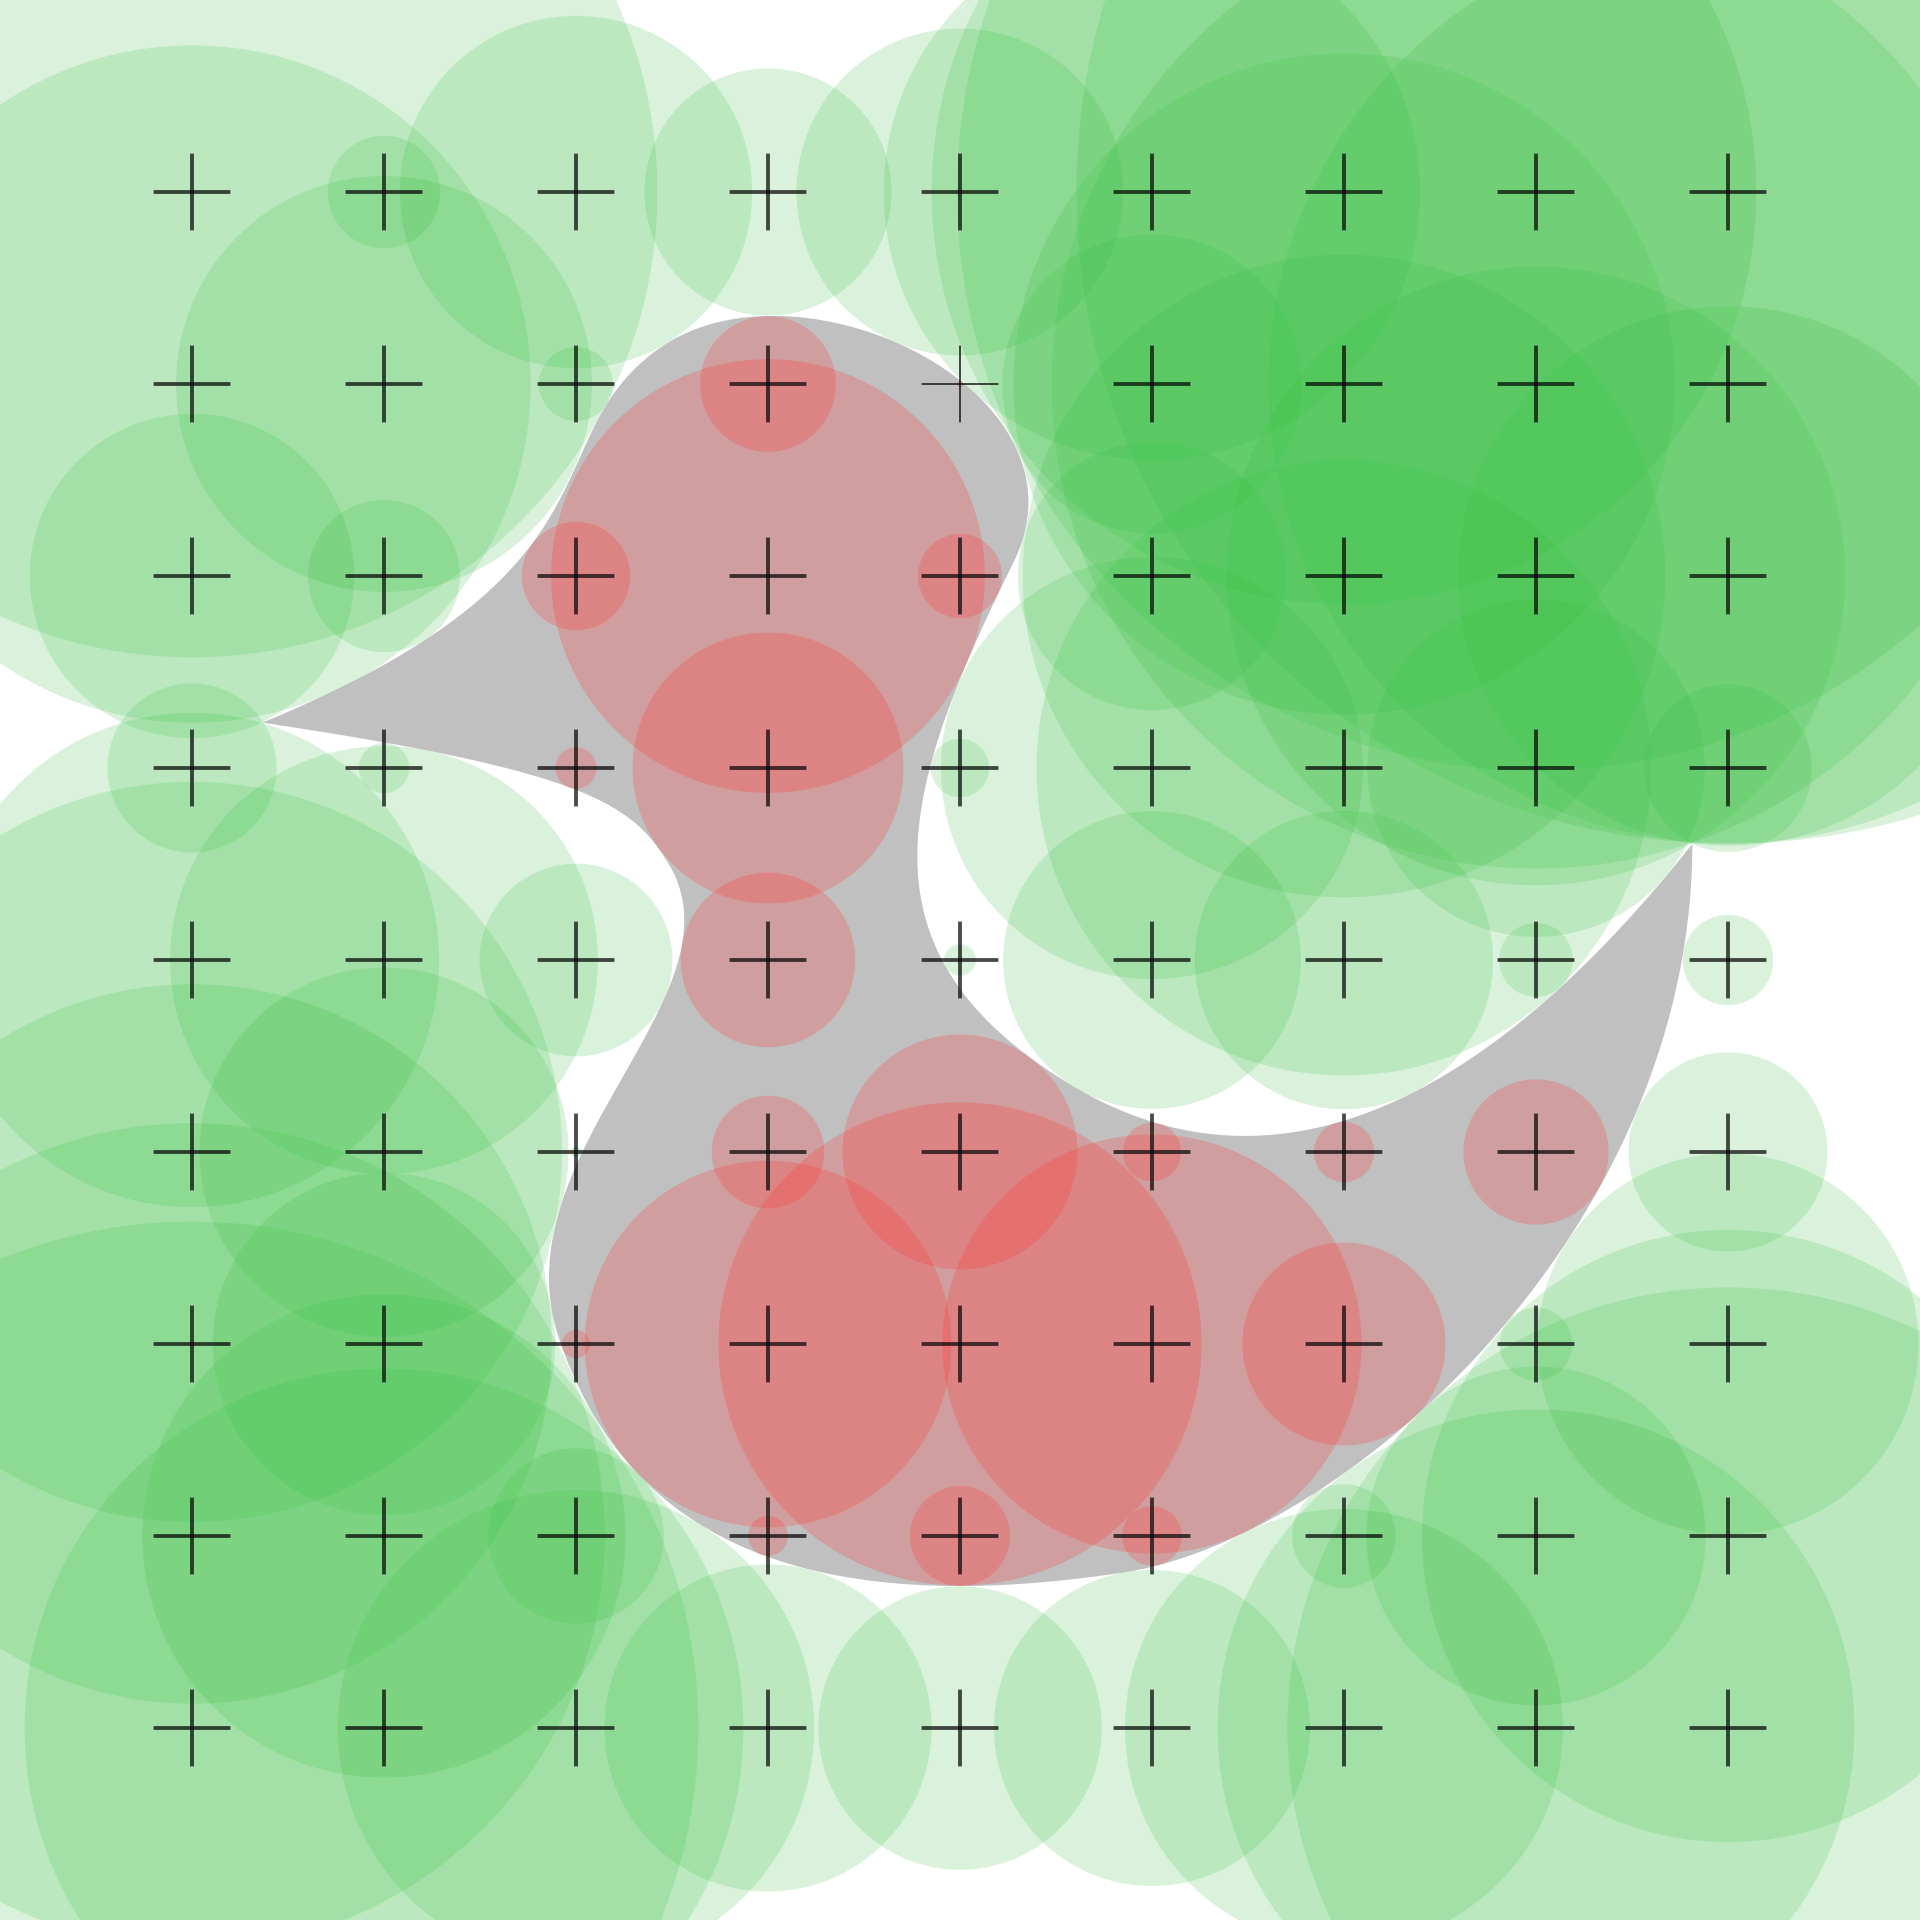
\includegraphics[width=0.5\linewidth]{figs/2d-sdf.png}
    \caption{An illustration of Signed Distance Function for a 2D metric space discretized into pixels (query coordinates '+') (Courtesy: Wikipedia).}%
    \label{fig:2d-sdf}
\end{figure}

\subsubsection{TSDF integration}

A TSDF representation requires a metric volume by design, which is implemented as a volumetric grid $V$, arbitrarily initialised in the world frame $\Tv_W = \Iv \in SE(3)$. Consider a single RGBD frame measurement $\langle \Ic, \Dc \rangle$ that consists of a color ($\Ic$) and depth ($\Dc$) image, at a relative camera pose $\Tv_C^W  = \begin{bmatrix}
    \Rv_C^W & \tv_C^W \\ 0 & 1
\end{bmatrix}\in SE(3)$ with camera intrinsics $\Kv$. To integrate the measurement into the TSDF volume, we project  all the query points $q \in \Rb^3$ of the volume $V$ into the current image as follows:
\begin{align}
    \dot{q}^\prime = (\Tv_C^W)^{-1} \dot{q} \\
    \dot{p} = \lfloor \Kv q^\prime\rfloor
\end{align}
where $\dot{q} = \begin{bmatrix}
    q^\top & 1
\end{bmatrix}^\top$  and similarly $\dot{p}$ denote the homogeneous coordinates in $\Rb^2$ and $\Rb^3$ respectively. $p \in \Zb^2$ is the associated 2D pixel coordinate in the image and $\lfloor \cdot \rfloor$ is the floor function and finds the greatest integer pixel coordinate less than the pixel value in the image. For every matched pixel coordinate, we backproject the associated measurement i.e., the depth value of the pixel $\Dc(p) \in \Rb$ into the volume to obtain a \emph{noisy} 3D surface in the metric space (see Figure~\ref{fig:tsdf-single-image}). This noisy surface is used as the proxy surface against which all query coordinates ($q \in \Zb^3$) in the volumetric grid are evaluated against to obtain their corresponding SDF values as follows:

\begin{align}
    \text{SDF}(q) =  \norm{ \Dc(p) - \frac{1}{\lambda} \|\tv_C^W - q\|_2 }_2
\end{align}

 where $\| \tv_C^W - q \|_2$ is the distance between the query point and the camera center along the camera optical axis, and $\lambda = K^{-1} p$ defines the ray direction for the pixel $p$. This effectively calculates the shortest distance of the query coordinate to the surface.

\begin{figure}[htpb]
    \centering
    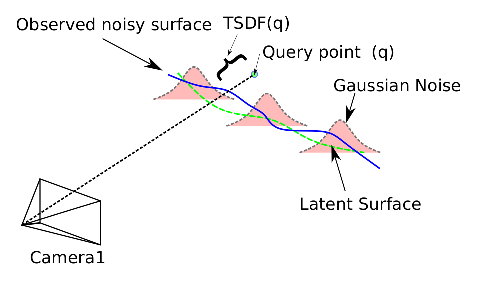
\includegraphics[width=0.6\linewidth]{figs/tsdf-integration-single}
    \caption{Back-projection of associated pixels into the 3D volumetric grid to obtain a noisy surface.}%
    \label{fig:tsdf-single-image}
\end{figure}

This SDF value is truncated such that only a band of SDF values ($+\mu$ to $-\mu$) around the measured surface are computed, to avoid computation of all the query coordinates in the volume.
Similarly, colors from the image can be associated to the query coordinates by unprojection uniquely since a depth image is available.

\begin{figure}[htpb]
    \centering
    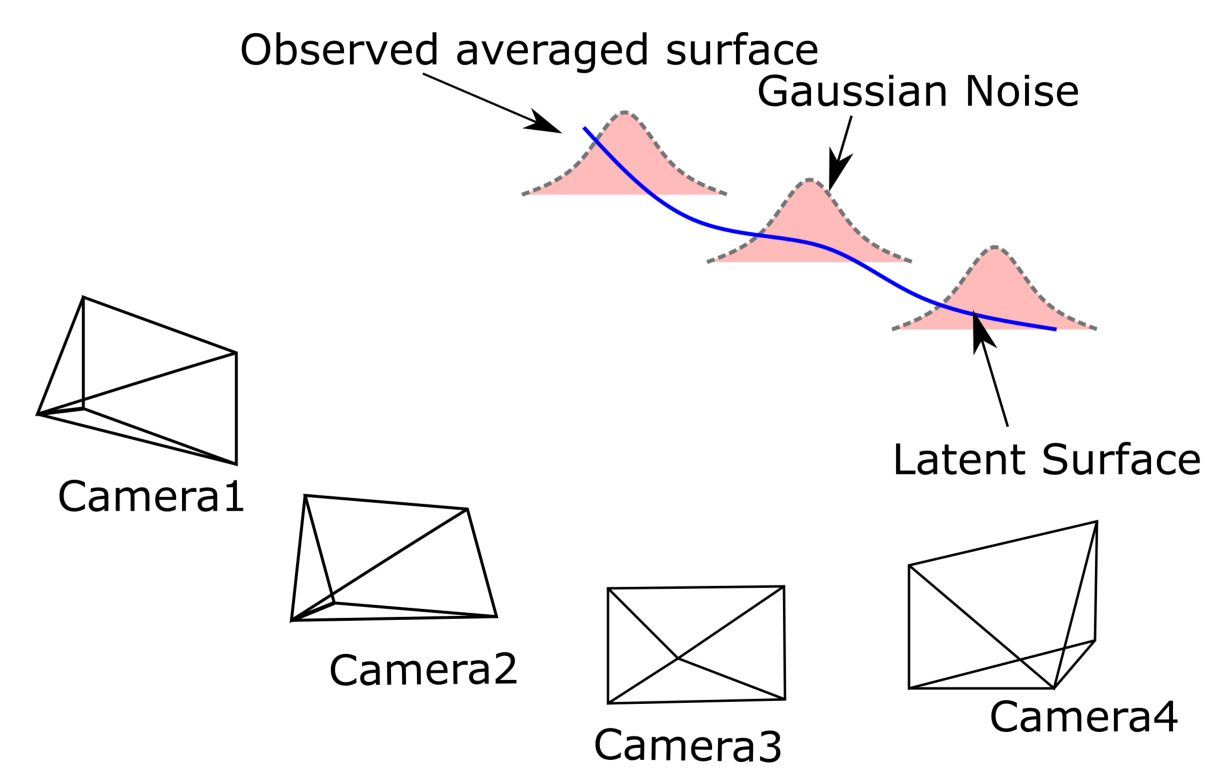
\includegraphics[width=0.5\linewidth]{figs/tsdf-multiple-images.png}
    \caption{On weighted averaging of TSDF values obtained from multiple RGBD measurements, in the limit we converge to TSDF values of the underlying surface.}%
    \label{fig:tsdf-multiple-images}
\end{figure}

Now, when we have multiple RGBD frame measurements $\{\langle \Ic^{(i)}, \Dc^{(i)} \rangle\}_{i=1}^{N}$ with their respective poses $\{ T_{C^{(i)}}^W \}_{i=1}^N$, we can compute TSDF measurements from each individual frame. The global fusion of all these TSDF measurements is then done through weighted average of the TSDF measurements for each query coordinate $q \in \Rb^3$ over the camera frame sequence as follows:
\begin{align}
    d &= \phi(\text{SDF}(q)) \\
    \text{TSDF}_k(q) &= \frac{\text{TSDF}_{k-1}(q) + d}{W(q) + 1} \\
    W(q) &= W(q) + 1
\end{align}
where $\phi$ truncates the $\text{SDF}$ computed for the frame being integrated, and $W(q)$ corresponds to the maintained weight for every voxel coordinate in the volume grid. This integration process intuitively results in evaluation of the SDF values for the query coordinates with the expected surface (mean of the TSDFs) from all the incorporated RGBD measurements (see Figure~\ref{fig:tsdf-multiple-images}).


In general, the integration process can also be applied to the color values, where the colors are averages elementwise, with the incoming stream of images.

\subsubsection{TSDF Rendering}

TSDF Rendering is the process of generating a virtual depth and color image given a camera pose $\Tv_C^W$ and TSDF volume grid $V$. The previous subsection assumed access to camera poses for global TSDF fusion, but in an actual SLAM setting camera poses are computed in the loop typically through iterative closest point (ICP)~\cite{rusinkiewiczEfficientVariantsICP2001} registration. TSDF Rendering is the intermediate step that generates a virtual image that the incoming camera frame is registered against (also called \emph{frame to model} registration~\cite{newcombeKinectFusionRealtimeDense2011}). (details in \S\ref{subsec: tracking})

Rendering is accomplished by marching a ray per pixel of the virtual frame into the global TSDF volume which encodes surfaces as the zero level set (zero crossing). For a given pixel $p \in \Zb^2$, once again the camera ray can be computed as
\begin{align*}
    \rv = \Tv_C^W \Kv^{-1} \dot{p}.
\end{align*}
\noindent We then march along the ray from the minimum depth supported by the camera (usually assumed to be $0.1$m) to a max depth value defined by the supported camera range (around 5m to 8m for Microsoft Kinect), or until we find a zero crossing. Typically this process is sped up by skipping marching along the ray, and using a step size $< \mu$, the truncation threshold. Once a zero crossing has been found, the depth value can be further refined by trilinear interpolation. (details in~\cite{newcombeKinectFusionRealtimeDense2011})

\subsection{TSDF Limitations}

Based on the discussion of TSDF for map representation in SLAM, the following limitations might be apparent to the keen reader.
\begin{enumerate}
    \item \textbf{TSDF representation is memory intensive:} A naive TSDF representation, utilizes a 3D volumetric grid to represent the scene -- typically  a voxel grid of resolution $512^3$ covering a bounded volume of about $4m^3$. This makes the entire system very memory intensive. Later works such as Voxel Hashing~\cite{niessnerRealtime3DReconstruction2013} and OctoMap \cite{hornungOctoMapEfficientProbabilistic2013} have tried to ameliorate this issue. In our implementation, we utilize this spatial hashing based TSDF implementation based on \cite{dongGPUAcceleratedRobust2019} to achieve memory efficiency.
    \item \textbf{TSDFs are computationally intensive:} During integration of an incoming frame, all pixels that are projectively associated to the 3D query coordinates are updated requiring about $640\times 480 = 307200$ operations for a VGA resolution image. Similarly, during TSDF rendering, each pixel to be rendered requires at most $\frac{\|d_{\max} - d_{\min}\|_2}{\mu}$ evaluations, where $\|d_{\max} - d_{\min}\|_2$ is the maximum ray length, and $\mu$ is the TSDF truncation width. Therefore, ray-casting is typically the most computationally intensive step in any dense RGBD SLAM system. Observing that each pixel is updated independent of others, a GPU can (and is) used to parallelize all TSDF operations, to obtain realtime operation.

\begin{figure}[htpb]
    \centering
    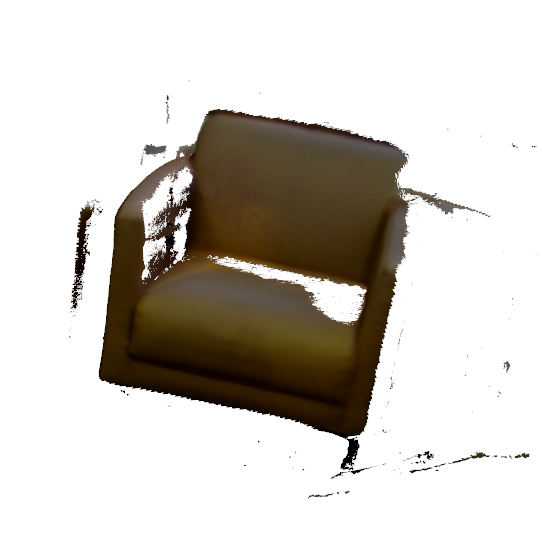
\includegraphics[width=0.4\linewidth]{figs/chair-landmark.png}
    \caption{An example of dense high level landmark in our SLAM system.}%
    \label{fig:chair-landmark}
\end{figure}

    \item \textbf{Cannot easily smooth noisy pose estimates:} It is not easy to correct noisy pose estimates with implicit models, and therefore most early systems employed only a filtering based integration \cite{newcombeKinectFusionRealtimeDense2011}. This is because to correct for a noisy pose estimate in retrospect requires the expensive operation of subtracting the weighted TSDF values in the global volume from the appropriate coordinates and re-integrating the volume with corrected TSDF values \cite{daiBundleFusionRealtimeGlobally2017}. \cite{whelanKintinuousSpatiallyExtended} used submaps to subvert this problem, however with large TSDF volumes as submaps there are still locally noisy measurements that are not corrected for. In our method, since we use a TSDF representation only for landmark objects, we reap the benefits of explicit representation, where the whole landmark pose can be optimized, but each landmark provides a dense and appealing representation. (see Figure~\ref{fig:chair-landmark})
\end{enumerate}

\section{The Back End}

The back end is responsible for generating a reasonable explanation in the state variables given the abstract sensor measurements and data associations from the front end. As opposed to filtering based methods such as Kalman Filter, more recently smoothing formulations based on matrix factorization have provided exact solutions in the linear case, and approximate but good solutions in non-linear case by adding the entire trajectory into the optimization problem while simplifying the solution~\cite{kaessIncrementalSmoothingMapping}. In this section, I review the batch smoothing formulation that is quite common in graph based SLAM back-ends today~\cite{grisettiTutorialGraphBasedSLAM, dellaertFactorGraphsRobot2017}.

\subsection{SLAM and Non-Linear Least Squares}

\begin{figure}[htpb]
    \centering
    \includegraphics[width=\linewidth]{figs/factor-graph-background}
    \caption{(a) A factor graph typical for SLAM and (b) the explicit Bayes net for the factor graph in (a). Note the Markovian conditional independences between measurements, given the state variables.}%
    \label{fig:factor-graph}
\end{figure}

As introduced in Chapter \ref{chap:introduction}, by treating the robot states and landmarks as random variables given measurements, the SLAM problem can be treated as the maximum a posteriori (MAP) estimation of robot and landmark states. Now, consider a collection of robot state variables $\Xc \triangleq \{ \xv_t \}_{t=1}^{T}$, and a collection of landmarks $\Lc \triangleq \{ \ell_m \}_{m=1}^{M}$, and set of measurements $\Zc \triangleq \{\{\zv_n \}_{n=1}^{N}, \{\zv_t\}_{t=1}^{T}\}$ including both landmark and odometry measurements respectively, then the MAP estimation is given as
\begin{align}
    \Xc^*, \Lc^* = \argmax_{\Xc, \Lc} p(\Xc, \Lc | \Zc) = \argmax_{\Xc, \Lc} p(\Zc | \Xc, \Lc) p(\Xc, \Lc) \label{eq:map}
\end{align}
While MAP estimation is known to be NP-Hard in general, by assuming reasonable conditional independences between the associated variables (see Figure~\ref{fig:factor-graph}), i.e., by making the markovian assumption on the state variables, and observing that measurements are local, we can write the joint probability in \ref{eq:map} as follows:
\begin{align}
    p(\Xc, \Lc, \Zc) &= p(\xv_0) \prod_{n=1}^{N} p(\zv_n | \xv_{\alpha_n}, \ell_{\beta_n}) \prod_{t=1}^{T} p(\zv_t | \xv_{t-1}, \xv_{t})\nonumber\\
    \log p(\Xc, \Lc, \Zc) &= \log p(\xv_0) + \sum_{n=1}^{N} \log p(\zv_n | \xv_{\alpha_n}, \ell_{\beta_n}) + \sum_{t=1}^{T} \log p(\zv_t | \xv_{t-1}, \xv_{t})
\end{align}
Note, that the above problem assumes known \emph{data association} between measurements $\zv_n$ of landmark $\ell_{\beta_n}$ at a robot pose $\xv_{\alpha_n}$as $\Dc := \{(\alpha_n, \beta_n)\}_{n=1}^{N}$ \cite{bowmanProbabilisticDataAssociation2017}.
Now as is typical in SLAM, we assume Gaussian measurement noise in each of the measurements i.e.,
\begin{align}
    \zv_0 &= \xv_0 + \nuv_0\\
    \zv_n &= h_n(\xv_{\alpha_n}, \ell_{\beta_n}) + \nuv_n\\
    \zv_t &= h_t(\xv_{t-1}, \xv_t) ~+ \nuv_t
\end{align}
Where $\nuv_n$ and $\nuv_t$ are the intrinsic noise in the respective measurements, each distributed as zero mean noise with respective covariances $\Sigma_n$ and $\Sigma_t$. Also note that we added a phantom measurement $\zv_0$ to constrain the first pose with an empirically chosen small covariance $\Sigma_0$. On writing down the probability distributions for each of the Gaussian noise terms we have the following:
\begin{align}
    p(\xv_0) &\propto \exp\{ \|\zv_0 - \xv_0\|^2_{\Sigma_0}\}\\
    p(\zv_n | \xv_{\alpha_n}, \ell_{\beta_n}) &\propto \exp\{ \|\zv_n - h_n(\xv_{\alpha_n}, \ell_{\beta_n})\|^2_{\Sigma_n}\}\\
    p(\zv_t | \xv_{t-1}, \ell_{t}) &\propto \exp\{ \|\zv_t - h_n(\xv_{t-1}, \ell_{t})\|^2_{\Sigma_t}\}
\end{align}
Observe that
\begin{align}
    \Xc^*, \Lc^* &= \argmax_{\Xc, \Lc} p(\Xc, \Lc, \Zc) = \argmin_{\Xc, \Lc} - \log p(\Xc, \Lc, \Zc)
\end{align}
Now writing the joint probability using the factorized measurement distributions we have
\begin{align*}
    \Xc^*, \Lc^* = \argmin_{\Xc, \Lc} \Bigg \{ \| \zv_0 - \xv_0 \|_{\Sigma_0}^2 + &\sum_{n=1}^{N} \| \zv_n - h_n(\xv_{\alpha_n}, \ell_{\beta_n}) \|_{\Sigma_t}^2 + \\&\sum_{t=1}^{T}\| \zv_t - h_t(\xv_{t-1}, \xv_{t}) \|_{\Sigma_n}^2 \Bigg \}
\end{align*}
If we generalize the different types of measurements in the system as $h_i(\Xv_i)$, and subsume the landmarks and state variables into a single state vector $\Xc$ then we may write the above as:
\begin{align}
    \Xc^* = \argmin_{\Xc} \Bigg \{ &\sum_{i=1}^{N} \| \zv_i - h_i(\Xv_i) \|_{\Sigma_i}^2 \Bigg \} \label{eq:least-squares}
\end{align}
The above minimization is a non-linear least squares optimization which is typically solved by iteratively linearizing the measurement models and solving a series of linear approximations to the problem to approach a local minima solution for landmark and robot latent state variables.

\subsection{Iterative Linearization and Gauss Newton}


Consider a single non-linear measurement $h_i( \cdot )$, then by Taylor's expansion, we can linearize the measurement at a linearization point $\Xv_i^{(0)}$ as follows (see Figure~\ref{fig:taylor}):
\begin{align}
    h_i(\Xv_i) \approx h_i(\Xv_i^{(0)}) + \frac{\partial h_i}{\partial \Xv_i} \Bigg |_{\Xv_i^{(0)}} (\Xv_i - \Xv_i^{(0)})
\end{align}
If we define the jacobian as $\Jv_i \triangleq \frac{\partial h_i}{\partial \Xv_i} \Big|_{\Xv_i^{(0)}}$, and $\Delta_i \triangleq (\Xv_i - \Xv_i^{(0)})$ and substitute in the general non-linear least squares objective \ref{eq:least-squares}:

\begin{figure}[htpb]
    \centering
    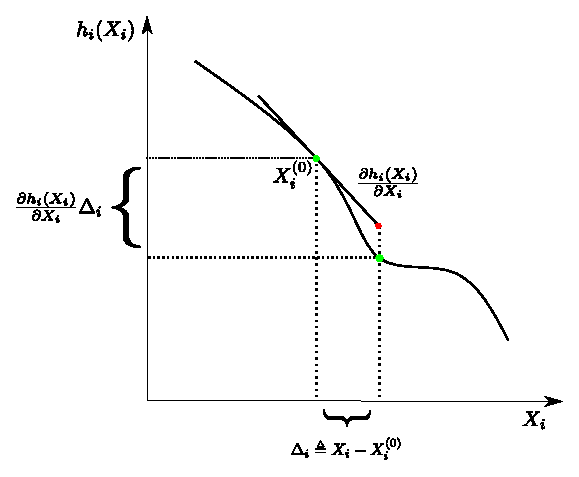
\includegraphics[width=0.5\linewidth]{figs/linearization}
    \caption{Illustration of linearization using Taylor's expansion.}
    \label{fig:taylor}
    \vspace{-1em}
\end{figure}
\begin{align}
    \Delta^* = \argmin_{\Delta}\sum_{i} \| \{\zv_i - h_i(X_i^{(0)})\} - \Jv_i \Delta_i \|_{\Sigma_i}^2
\end{align}
where $\qv_i \triangleq \zv_i - h_i(\Xv_i^{(0)})$ is the prediction error at the linearization point, and $\Delta^*$ is the solution to the locally linearized problem. Now we may write the least squares objective as:
\begin{align}
    \Delta^* &= \argmin_{\Delta}\sum_{i} \| \qv_i - \Jv_i \Delta_i \|_{\Sigma_i}^2 = \argmin_{\Delta}\sum_{i} (\qv_i - \Jv_i \Delta_i)^\top \Sigma_i^{-1} (\qv_i - \Jv_i \Delta_i)\\
             &=  \argmin_{\Delta}\sum_{i} \left\{\Sigma_i^{-1/2}(\qv_i - \Jv_i \Delta_i)\right\}^\top \left\{ \Sigma_i^{-1/2} (\qv_i - \Jv_i \Delta_i)\right\}\\
             &= \argmin_{\Delta}\sum_{i} \| \bv_i - \Av_i \Delta_i \|_2^2 = \argmin_{\Delta} \| \bv - \Av \Delta\|_2^2
\end{align}
By writing $\bv_i = \Sigma_i^{-1/2} \qv_i$ and $\Av_i = \Sigma_i^{-1/2} \Jv_i$ and then collecting them in the vector $\bv$ and matrix $\Av$ respectively, we obtain the standard least squares problem, that can then be solved using \emph{normal equations}.

The above solution gives us the local update $\Delta^*$ for a linearization point $\Xv^{(0)}$. To solve a non-linear problem, we solve for local updates iteratively as in Algorithm~\ref{gauss-newton}.


\begin{algorithm}[htpb]
\begin{algorithmic}[1]
    \Procedure{Gauss Newton}{$g(\Xv), \Xv^{(0)}$}
    \State $d = \text{threshold}$
    \For{t = 0 to N}
        \State $\Av, \bv \leftarrow$ Linearize$(g(\Xv))$ at $\Xv^{(t)}$
        \State $\Delta^* \leftarrow (\Av^\top \Av)^{-1} \Av^\top \bv$ \Comment{using QR or Cholesky factorization}
        \State $\text{temp} \leftarrow \Xv^{(t)} + \Delta^*$
        \If{$g(\text{temp}) < g(\Xv^{(t)})$}
            \State $\Xv^{(t+1)} \leftarrow \text{temp}$
            \If{$g(\Xv^{(t+1)}) - g(\Xv^{(t)}) < d$}
                \State \textbf{break}
            \EndIf
        \EndIf
    \EndFor
    \State \Return $\Xv^{(t)}$
\EndProcedure
\end{algorithmic}
\caption[short caption]{Iterative Non-linear optimization}
\label{gauss-newton}
\end{algorithm}


A more detailed treatment of sophisticated non-linear optimization algorithms in the context of SLAM is provided in \cite{dellaertFactorGraphsRobot2017}.

\subsection{Discussion and Limitations}

We noted earlier that MAP inference on the factor graph for the SLAM setting is tractable due to the inherent local structure of the factor graph. This structure appears in the sparsity of the measurement Jacobian $\Av = \Sigma^{-1/2} \Jv$ with number of rows equal to the number of measurements in the graph (number of factors) and the number of columns equal to the number of state variables to be solved. The non-linear least squares optimization is solved efficiently using matrix factorization methods such as QR factorization and Cholesky factorization (equivalent to variable elimination on the factor graph~\cite{dellaertSquareRootSAM2006}). Further improvement in performance can be gained by reordering the measurements using methods such as COLAMD \cite{davisAlgorithm8xxCOLAMD} which consequently reduces fill in in the matrix during computation.

Nevertheless, for an online system with this formulation matrix factorization needs to be performed with a new graph when new measurements are added, resulting in wasted computation to resolve all the entries in the matrix. Later work has made progress on incremental solvers for SLAM, that are able to update the solution iteratively for non-linear systems and provide linearization point management, as well as careful updation of older variables based on the current estimate. As this thesis does not directly use incremental solvers, the reader is directed to \citet{kaessISAM2IncrementalSmoothing2012}

For implicit mapping representations, however, it is unclear how they are to be represented as landmark variables, and how updates to the landmark state variables are to be propagated in the map. In this thesis, we show that representing the map as a collection of high level objects, each represented with implicit representation and corresponding to a landmark variable in the optimization is a good strategy, and benefits the SLAM in multiple facets. Each object is represented with a spatially hashed TSDF volumetric grid \cite{prisacariuInfiniTAMV3Framework2017} \cite{niessnerRealtime3DReconstruction2013} \cite{dongGPUAcceleratedRobust2019} that is not updated in the back end optimization process. Instead, since the object is rigid, optimizing the pose of the base frame attached to it suffices.
\clearpage
% In theory implicit map representations provide a method for water tight  reconstructions that are visually appealing, and in general more detailed when compared to feature based methods (see Figure Figure~\ref{fig:}), however these methods typically do not employ smoothing based back ends, and therefore are unable to correct for noisy pose estimates in retrospect. This is because, it is not easy to make a correction to an integrated measurement in the TSDF representation. In particular, to correct a single pose estimate, the measurement that had been integrated into the global TSDF has to be removed by subtractingthe corresponding TSDF value from the affected 3D query coordinates, and then re-integrating the new measurement appropriately.

